\section{Ejercicio 8}

Presentamos el siguiente lote corrido con distintos semillas de aleatoridad y tamaño de quantum.
El objetivo es mostrar que al ser pseudo-random, la semilla no produce favoritismo entre los procesos y que los diferentes quantum no van a alterar el fairness del algoritmo

*6 TaskBatch 20 5 \\

Hacer procesos largos iguales cortarlos antes de terminar y ver que el tiempo de CPU de cada uno tiende a igual, y que si veo màs que antes se mantiene, 
entonces da que es un scheduler "fairness"

Ver ejemplos de entrada salida y ver que estos tienden a tener mas CPU que los otros ya que la probabilidad aumenta por tener màs tickets\\

Semilla de Aleatoridad = 1 y Quantum = 3
\begin {center}
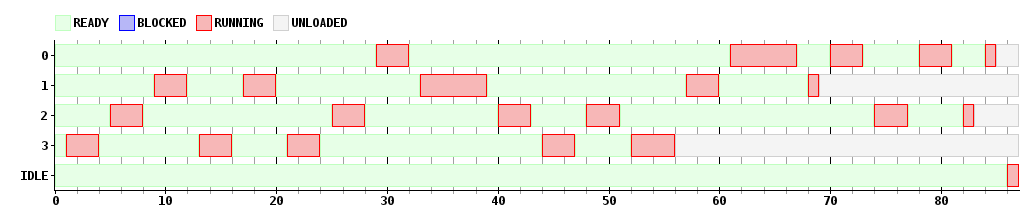
\includegraphics[width=16cm]{../simusched/outputs/ej8/sl-ej8-1-3.png}
\end {center}
Se puede ver en este ejemplo que si tomamos sectores de la corrida, vemos como la obtención de recursos se mantiene constante.\\
Tomemos los casos de 0 a 40, de 40 a 80 y 80 a 120.\\
De 0 a 40: el primer proceso obtiene \\
De 40 a 80:                           \\
De 80 a 120:                          \\

La concentración en la primera parte y después en la segunda

Semilla de Aleatoridad = 5 y Quantum = 2
\begin {center}
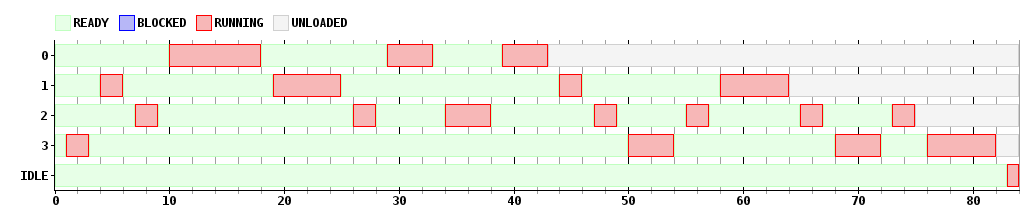
\includegraphics[width=16cm]{../simusched/outputs/ej8/sl-ej8-5-2.png}
\end {center}
Semilla de Aleatoridad = 3 y Quantum = 5
\begin {center}
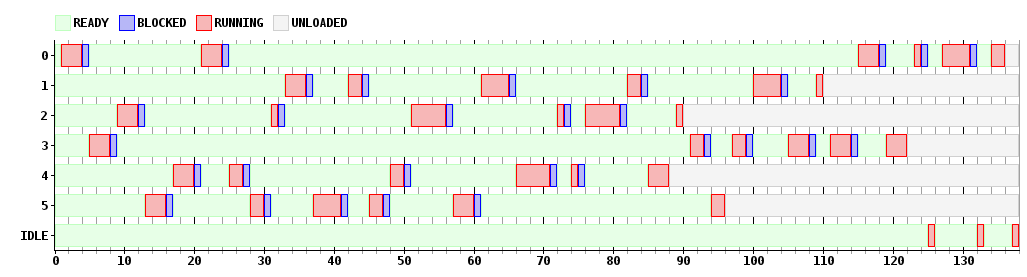
\includegraphics[width=16cm]{../simusched/outputs/ej8/sl-ej8-3-5.png}
\end {center}
Semilla de Aleatoridad = 4 y Quantum = 7
\begin {center}
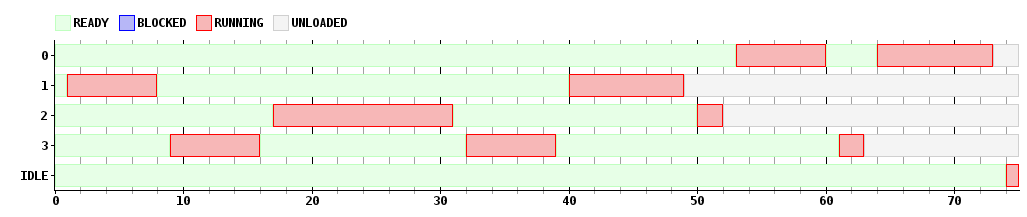
\includegraphics[width=16cm]{../simusched/outputs/ej8/sl-ej8-4-7.png}
\end {center}
Hasta acá es tipo Round robin ver de sacar algunos
Semilla de Aleatoridad = 2 y Quantum = 12
\begin {center}
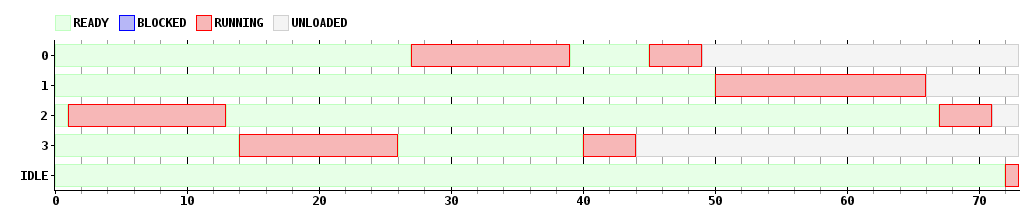
\includegraphics[width=16cm]{../simusched/outputs/ej8/sl-ej8-2-12.png}
\end {center}
Acá gano mucho la lotería, por algo es probabilisitoc

Para los I/O, ver que pasa lo mismo que en el anterior

Con estos mismos casos, se puede denotar como el algoritmo tiende a que los procesos obtengan en misma proporción el recurso.

Se puede notar que aunque se elija el mismo lote, la aleatoridad del algoritmo muestra como aunque se asignen de distinta forma los recursos, todos los procesos
tienden a obtenerlos uniformemente, siendo igualemente un algoritmo probabilìstico.\\

Cuenta tiempo de espera para cada gantt y ver que son parecido


Utilizamos el mismo ejemplo para notar la $"$compensación$"$. Notese como en el A el proceso 1 después de haber bloqueado 2 veces obtuvo tantos tickets que casi tuvo
exclusividad del procesador. Por el contrario el proceso 4 tuvo que esperar varios sorteos hasta salir ganador.
